In this chapter we will show the experiments made and their results, which we will also discuss. Most graphs were generated with Seaborn, the instance space graphics were generated with Bokeh.

\section{Experiments} \label{sec:experiments}

In the code, we define an experiment with a YAML configuration file. The file defines the number of output features in each layer, the number of training epochs and parameters for the optimizer. The next sections will define the experiments and show their results.

\subsection{Original Instance Space and region of data generation}

Figure \ref{fig:is_original} shows the original instance space with the parameters defined in Chapter \ref{ch:methodology}. We will be generating data in the region defined by a rectangle with vertices $(-2.0, -1.0)$ and $(-1.0, 0.0)$.

\begin{figure}[H]
    \centering
    \includegraphics[width=0.8\textwidth]{Cap5/is_original.png}
    \caption{Original instance space}
    \label{fig:is_original}
\end{figure}

\subsection{Experiment 1}

The first experiment is a simple encoder-decoder with 3 layers, with a list of layer output features being $[16, 8, 4]$. The parameters for the optmizer are a learning rate of 0.001 and a weight decay of 0.001, being trained for 50 epochs. The training epoch loss results from TensorBoard are shown in Figure \ref{fig:exp1}.

\begin{figure}[H]
    \centering
    \includegraphics[width=0.7\textwidth]{Cap5/loss_exp1}
    \caption{Experiment 1 training epoch loss}
    \label{fig:exp1}
\end{figure}

The loss has reduced nicely over the training epochs. Figure \ref{fig:is_gen_points1} shows the original instance space and the points generated in it.

\begin{figure}[H]
    \centering
    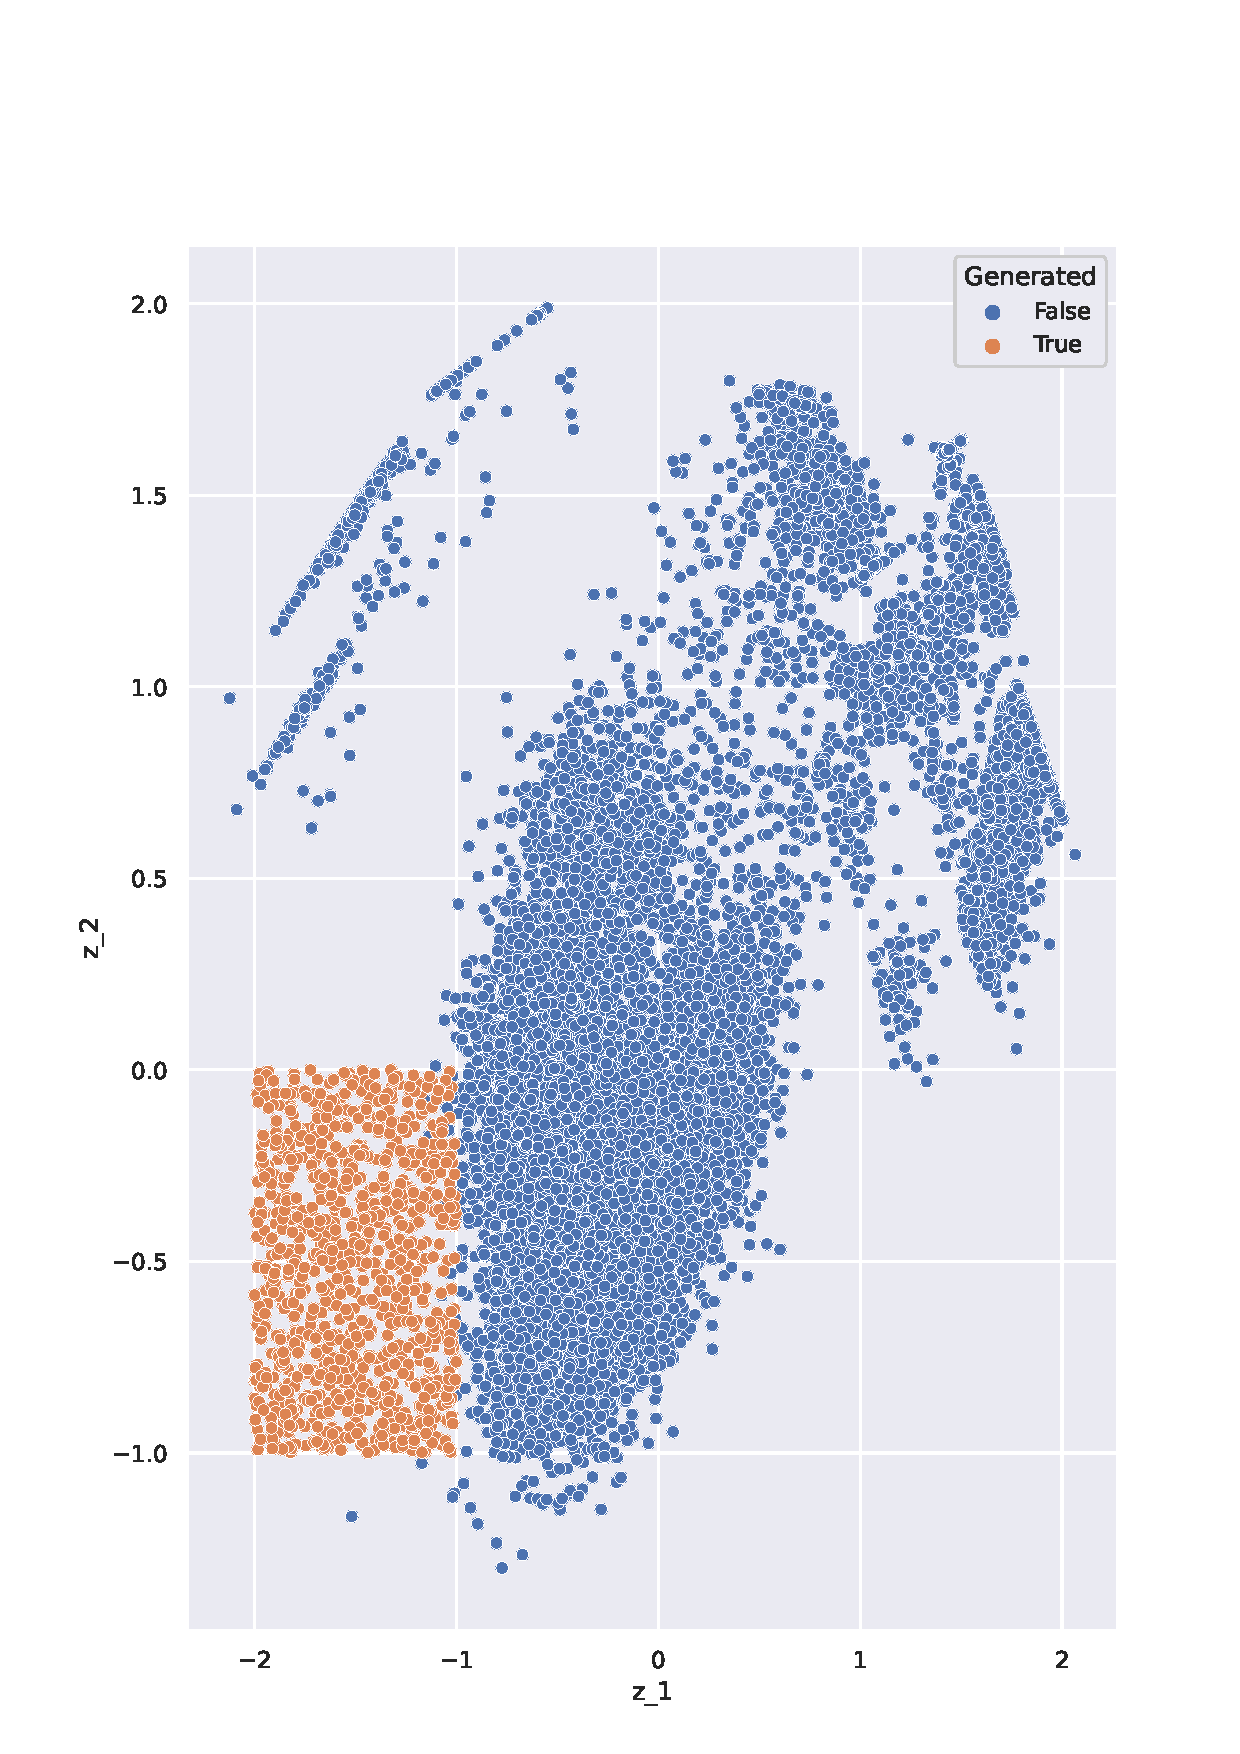
\includegraphics[width=0.8\textwidth]{Cap5/is_exp1.png}
    \caption{Instance space with generated points of experiment 1}
    \label{fig:is_gen_points1}
\end{figure}

Figure \ref{fig:is_exp1} shows the instance space with the points calculated from the generated meta-features. The points are not in the position we expected.

\begin{figure}
    \centering
    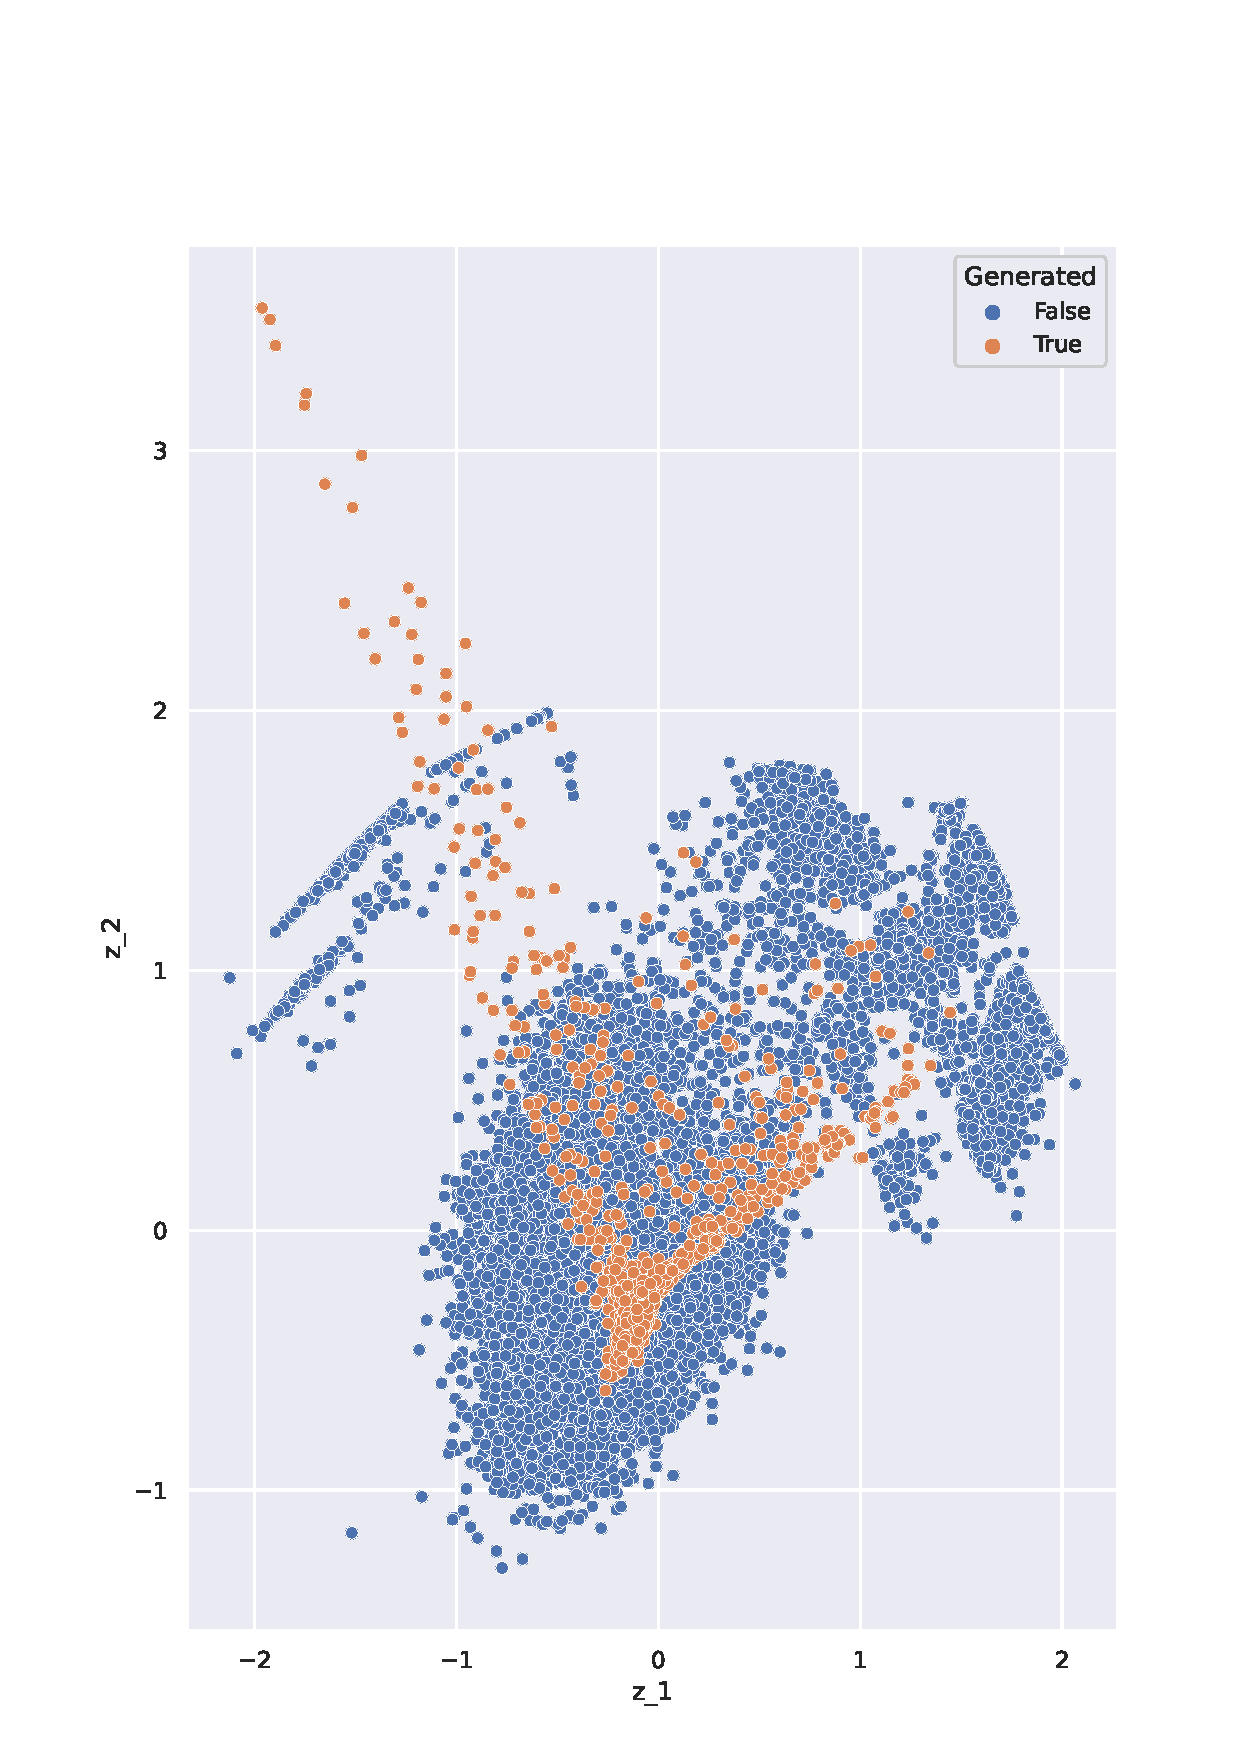
\includegraphics[width=0.7\textwidth]{Cap5/all_coords1.png}
    \caption{Instance space after calculating the position of the generated meta-features of the points generated in experiment 1}
    \label{fig:is_exp1}
\end{figure}

Figure \ref{fig:scatter_exp1} shows an scatterplot of the calculated instance space position value for each dimension versus the original generated value, with the colorbar representing the squared error of each point.

\begin{figure}[H]
    \centering
    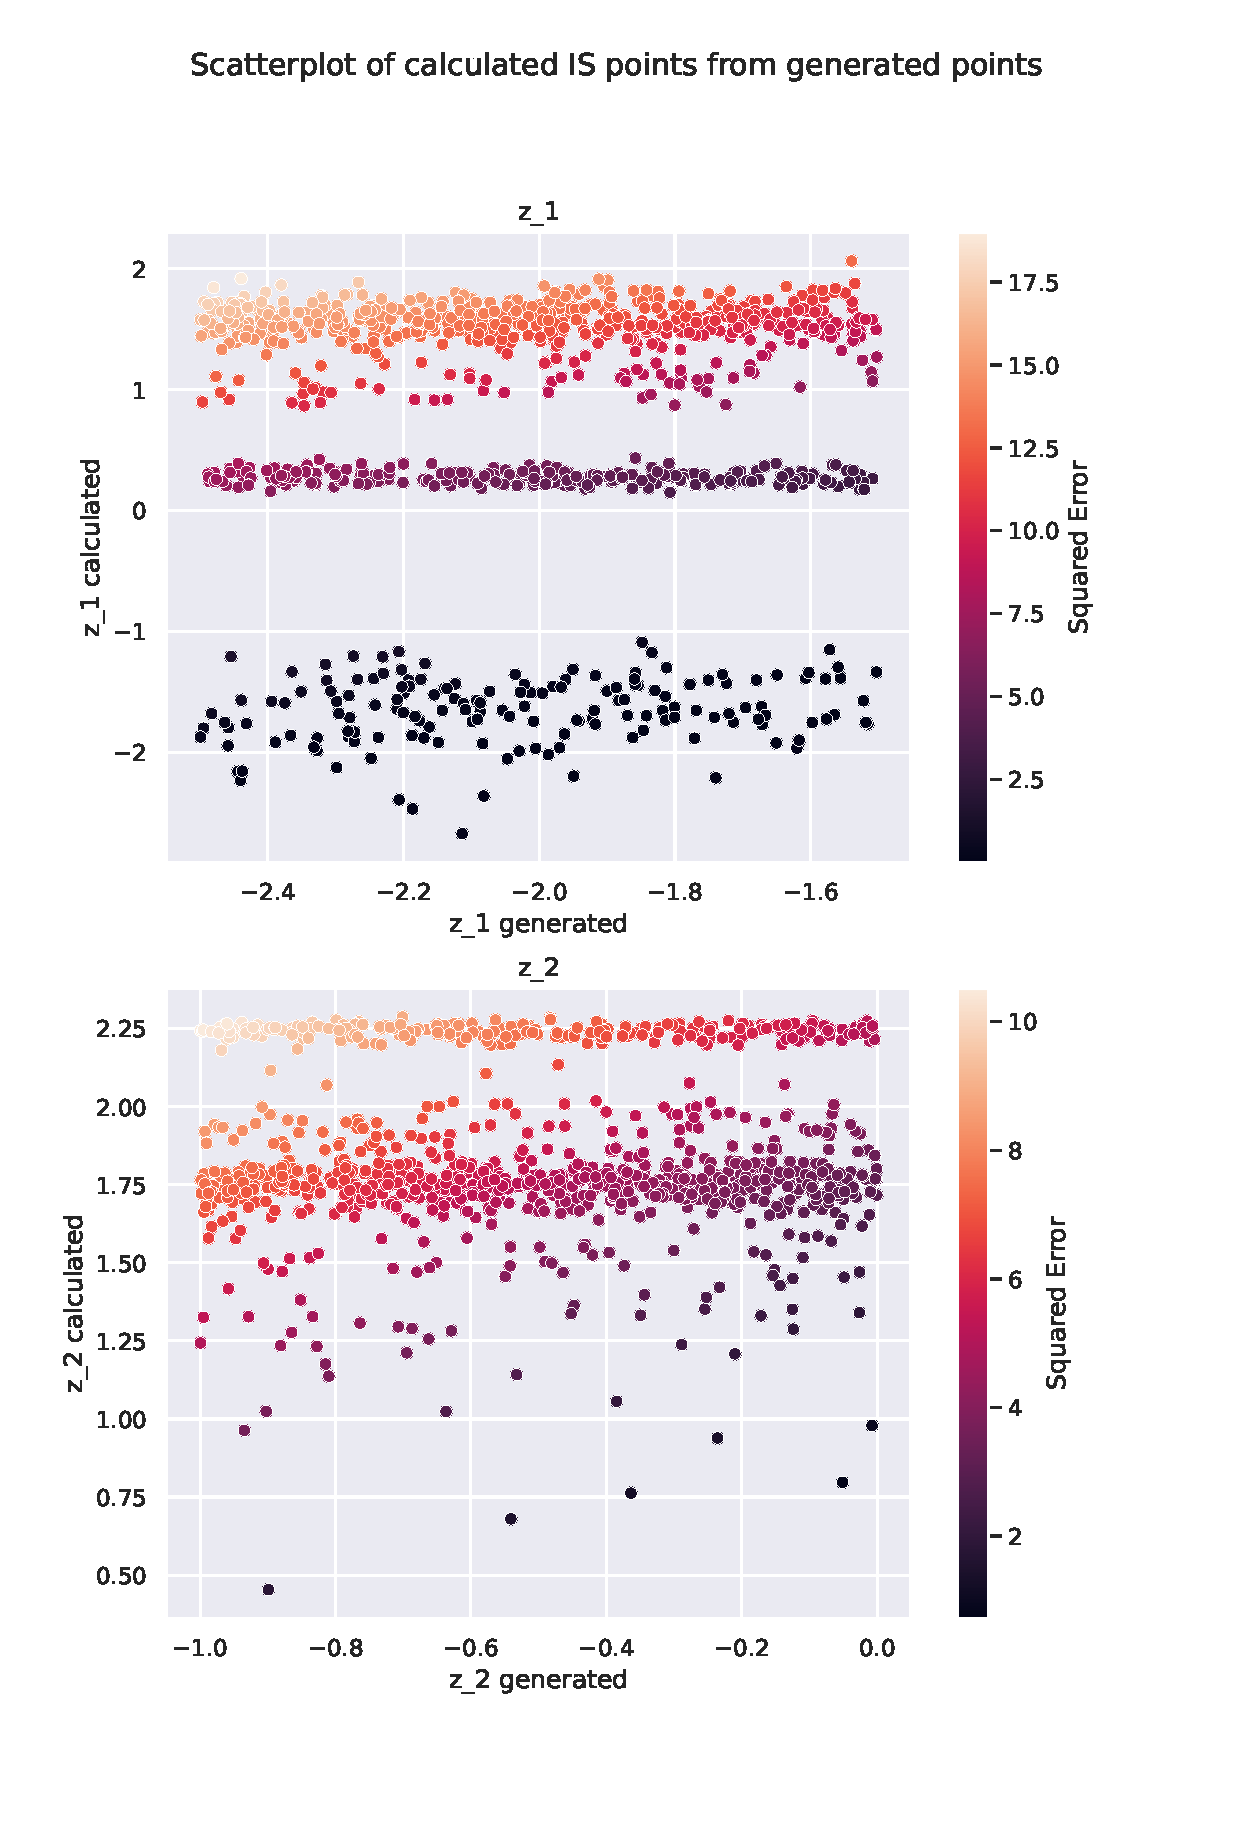
\includegraphics[width=0.7\textwidth]{Cap5/scatterplot1}
    \caption{Scatterplot of experiment 1}
    \label{fig:scatter_exp1}
\end{figure}

The calculated IS values are uncorrelated with the original values. This is a sign that the model is not working as intended. Figure \ref{fig:scatter_enc_exp1} shows the same scatterplot but for the calculated points against the points returned by the encoder, which are also uncorrelated.

\begin{figure}[H]
    \centering
    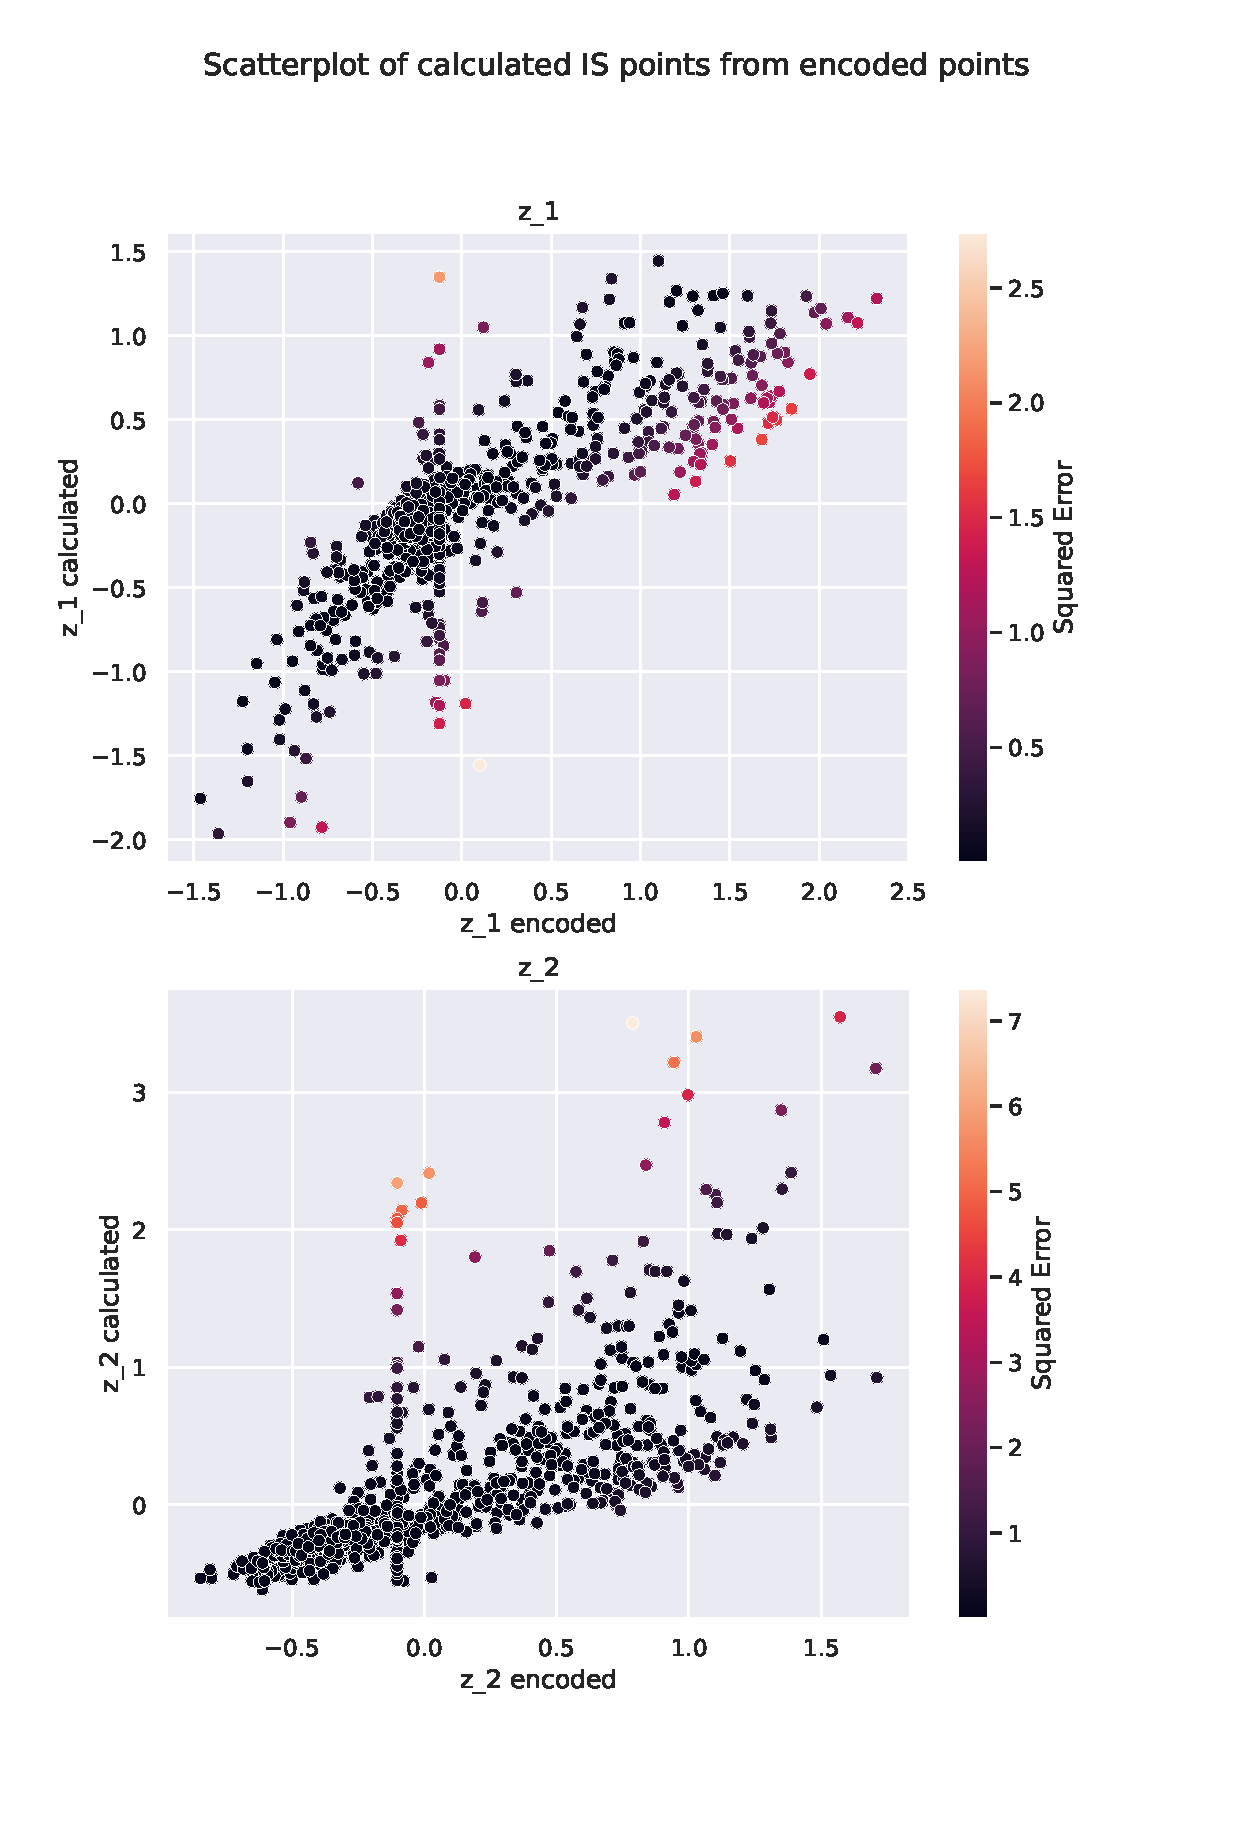
\includegraphics[width=0.7\textwidth]{Cap5/scatterplot_enc1}
    \caption{Scatterplot of experiment 1 encoder}
    \label{fig:scatter_enc_exp1}
\end{figure}

\subsection{Experiment 2}

In this experiment, we have two more layers and the output features are the list $[128, 32, 16, 8, 4]$. The optimizer parameters are the same, but the training epochs were reduced to 40. The training epoch loss results from TensorBoard are shown in Figure \ref{fig:exp2}.

\begin{figure}[H]
    \centering
    \includegraphics[width=0.7\textwidth]{Cap5/loss_exp2}
    \caption{Experiment 2 training epoch loss}
    \label{fig:exp2}
\end{figure}

The loss has reduced nicely over the training epochs as well. Figure \ref{fig:is_gen_points2} shows the instance space with the generated points. 

\begin{figure}[H]
    \centering
    \includegraphics[width=0.8\textwidth]{Cap5/is_exp2.png}
    \caption{Instance space with generated points of experiment 2}
    \label{fig:is_gen_points2}
\end{figure}


Figure \ref{fig:is_exp2} shows the instance space with the calculated points from the generated meta-features, with Figure \ref{fig:scatter_exp2} showing another scatterplot of the dimensions.

\begin{figure}[H]
    \centering
    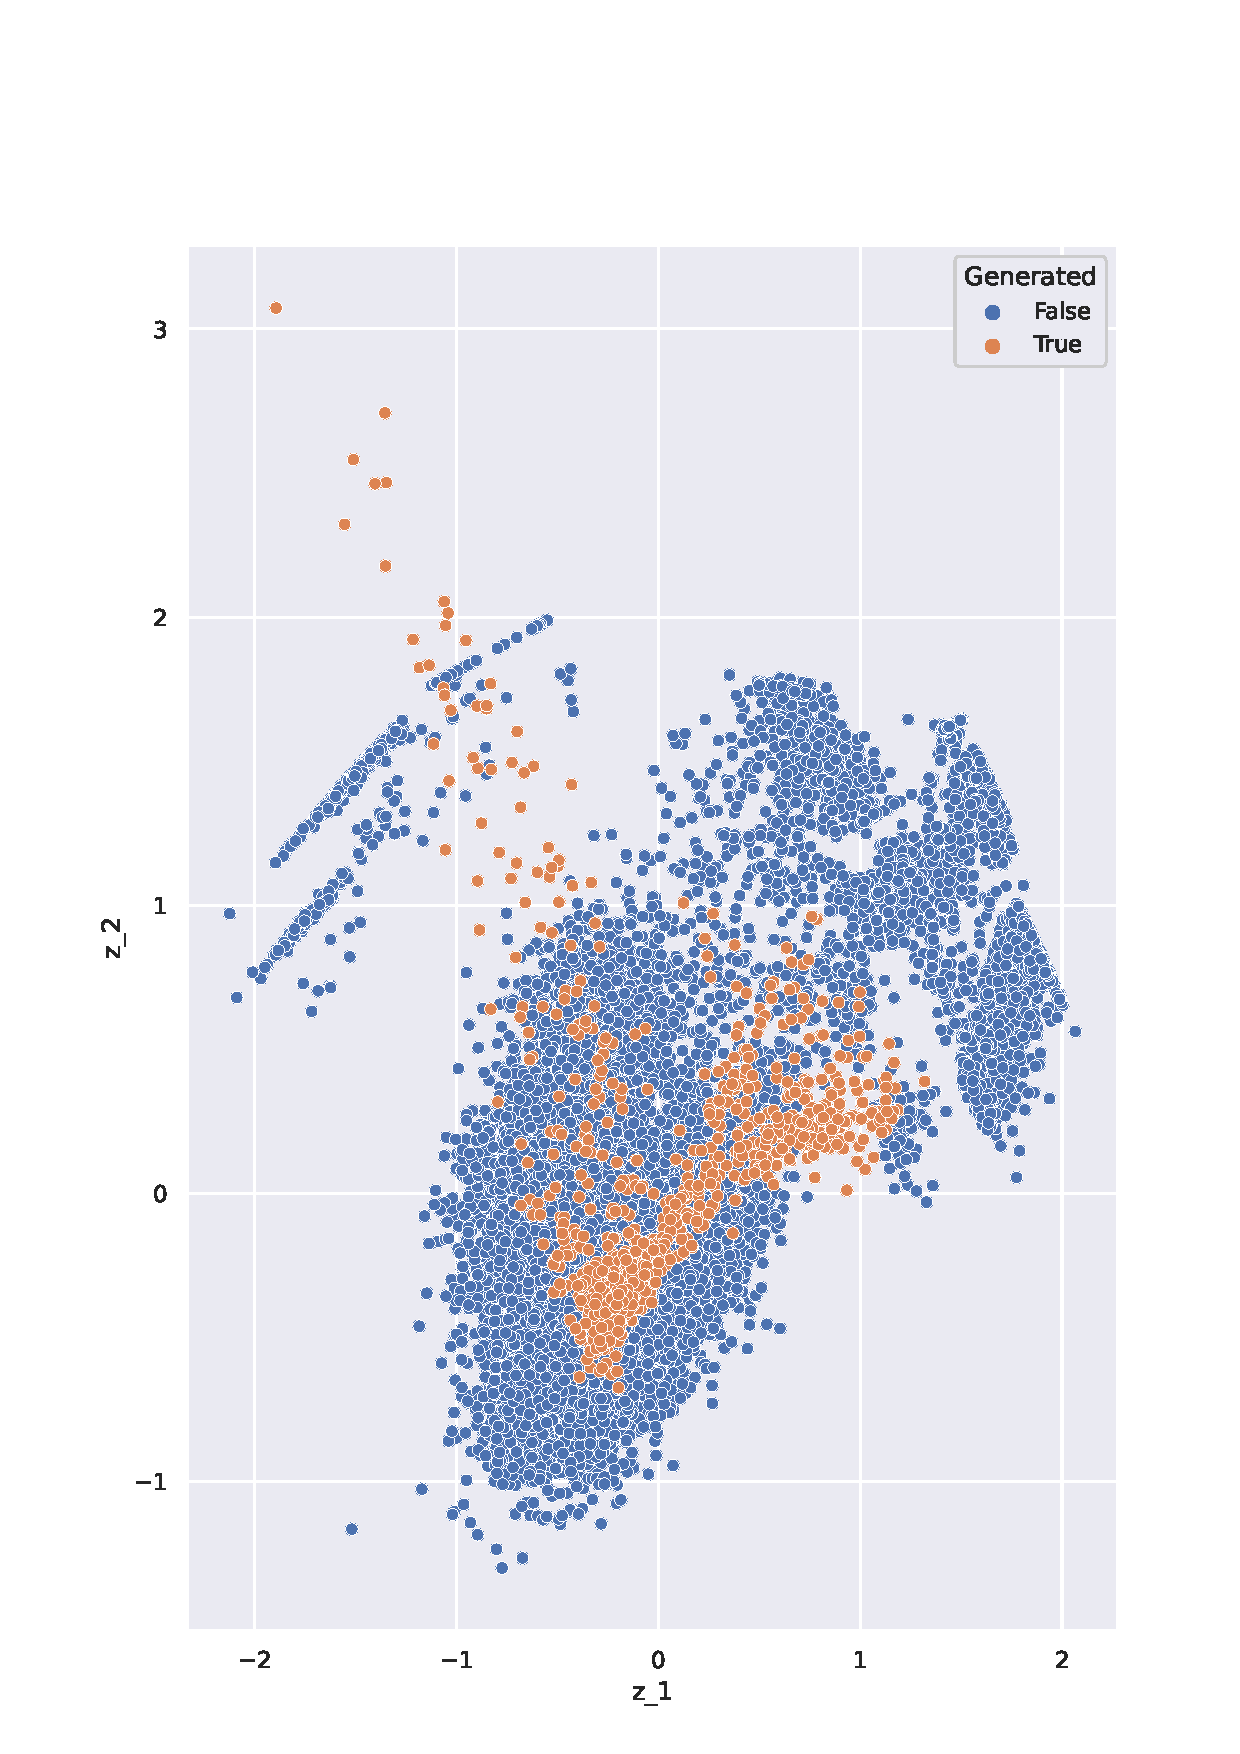
\includegraphics[width=0.8\textwidth]{Cap5/all_coords2.png}
    \caption{Instance space of experiment 2}
    \label{fig:is_exp2}
\end{figure}

\begin{figure}[H]
    \centering
    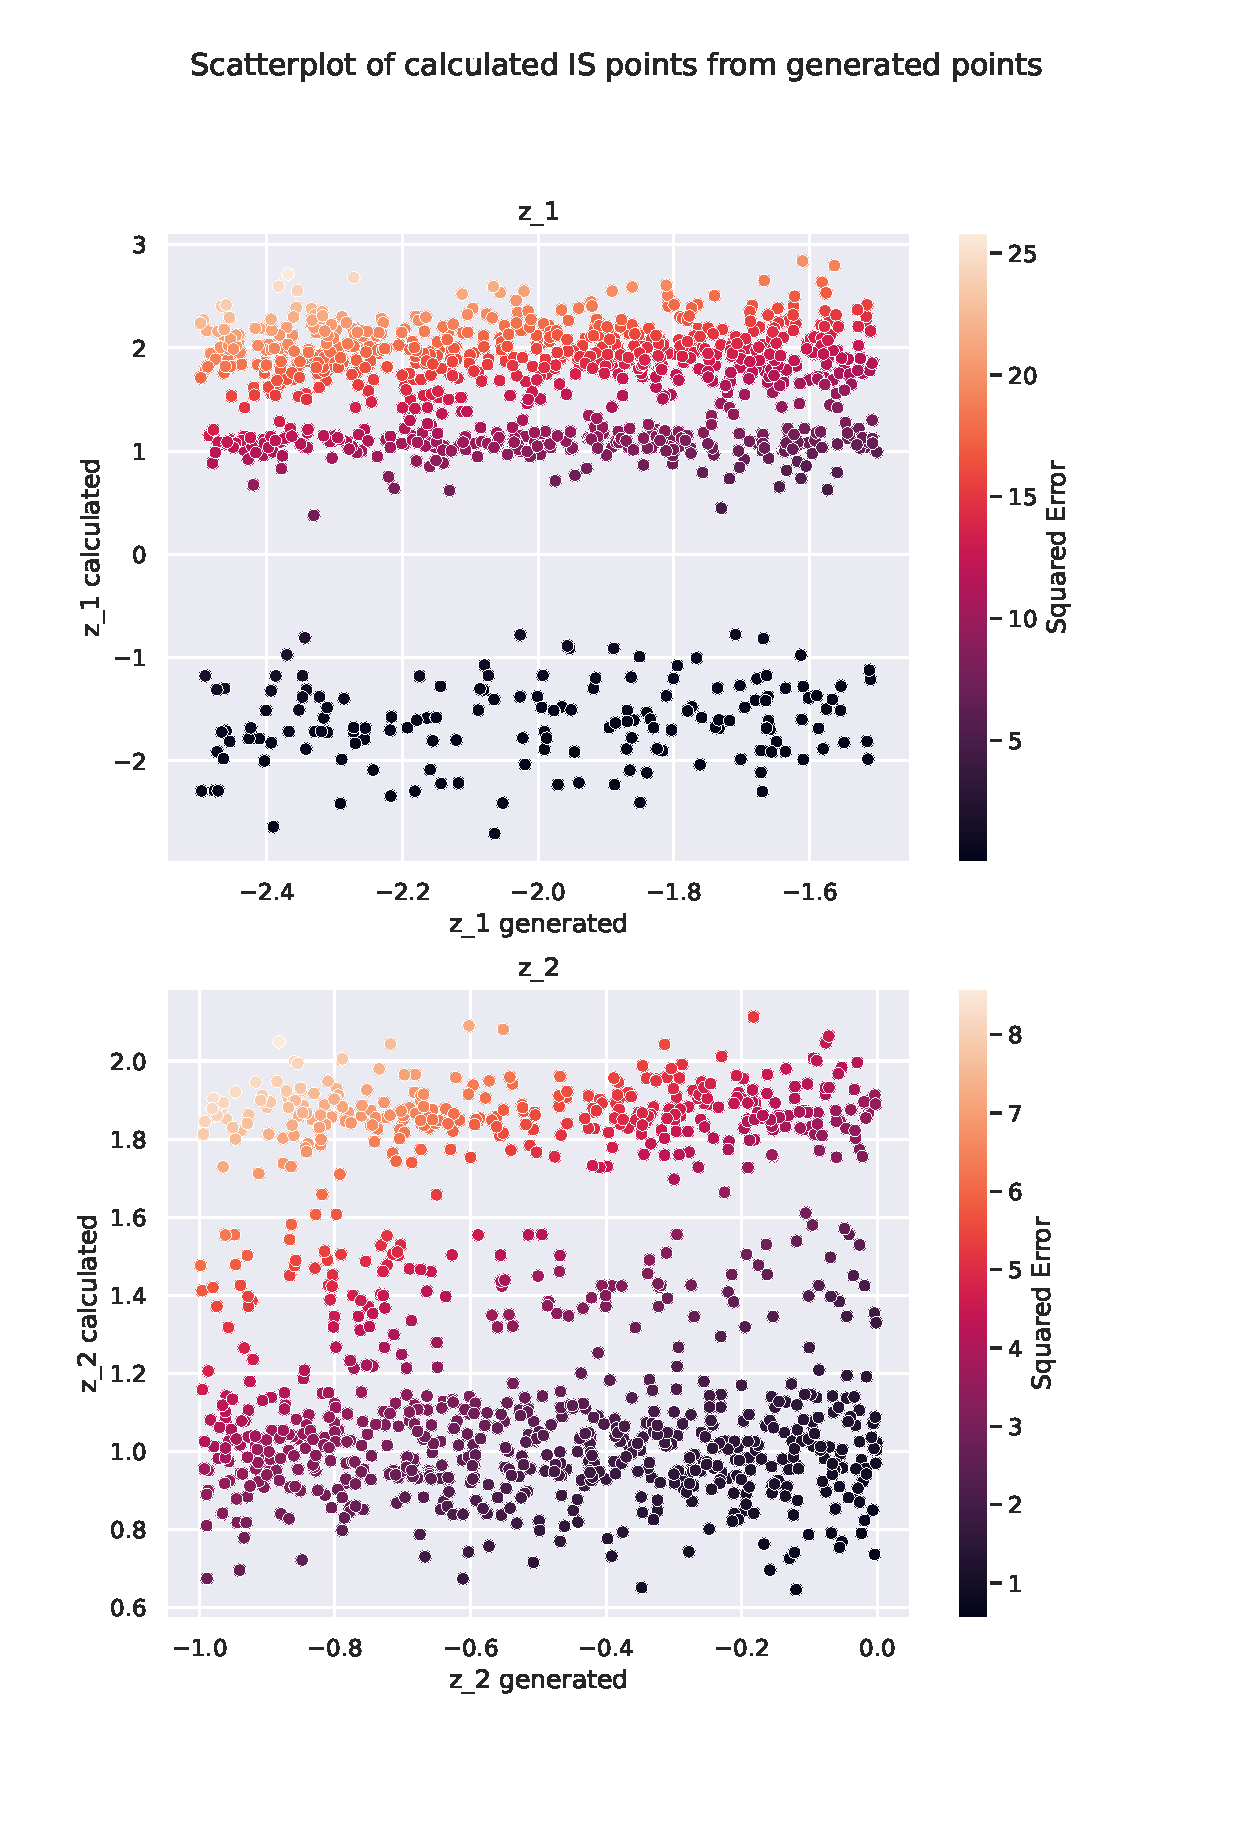
\includegraphics[width=0.7\textwidth]{Cap5/scatterplot2}
    \caption{Scatterplot of experiment 2}
    \label{fig:scatter_exp2}
\end{figure}

The calculated IS values are again uncorrelated with the original values. Figure \ref{fig:scatter_enc_exp2} shows the scatterplot for the points returned by the encoder. Again, they are uncorrelated.

\begin{figure}[H]
    \centering
    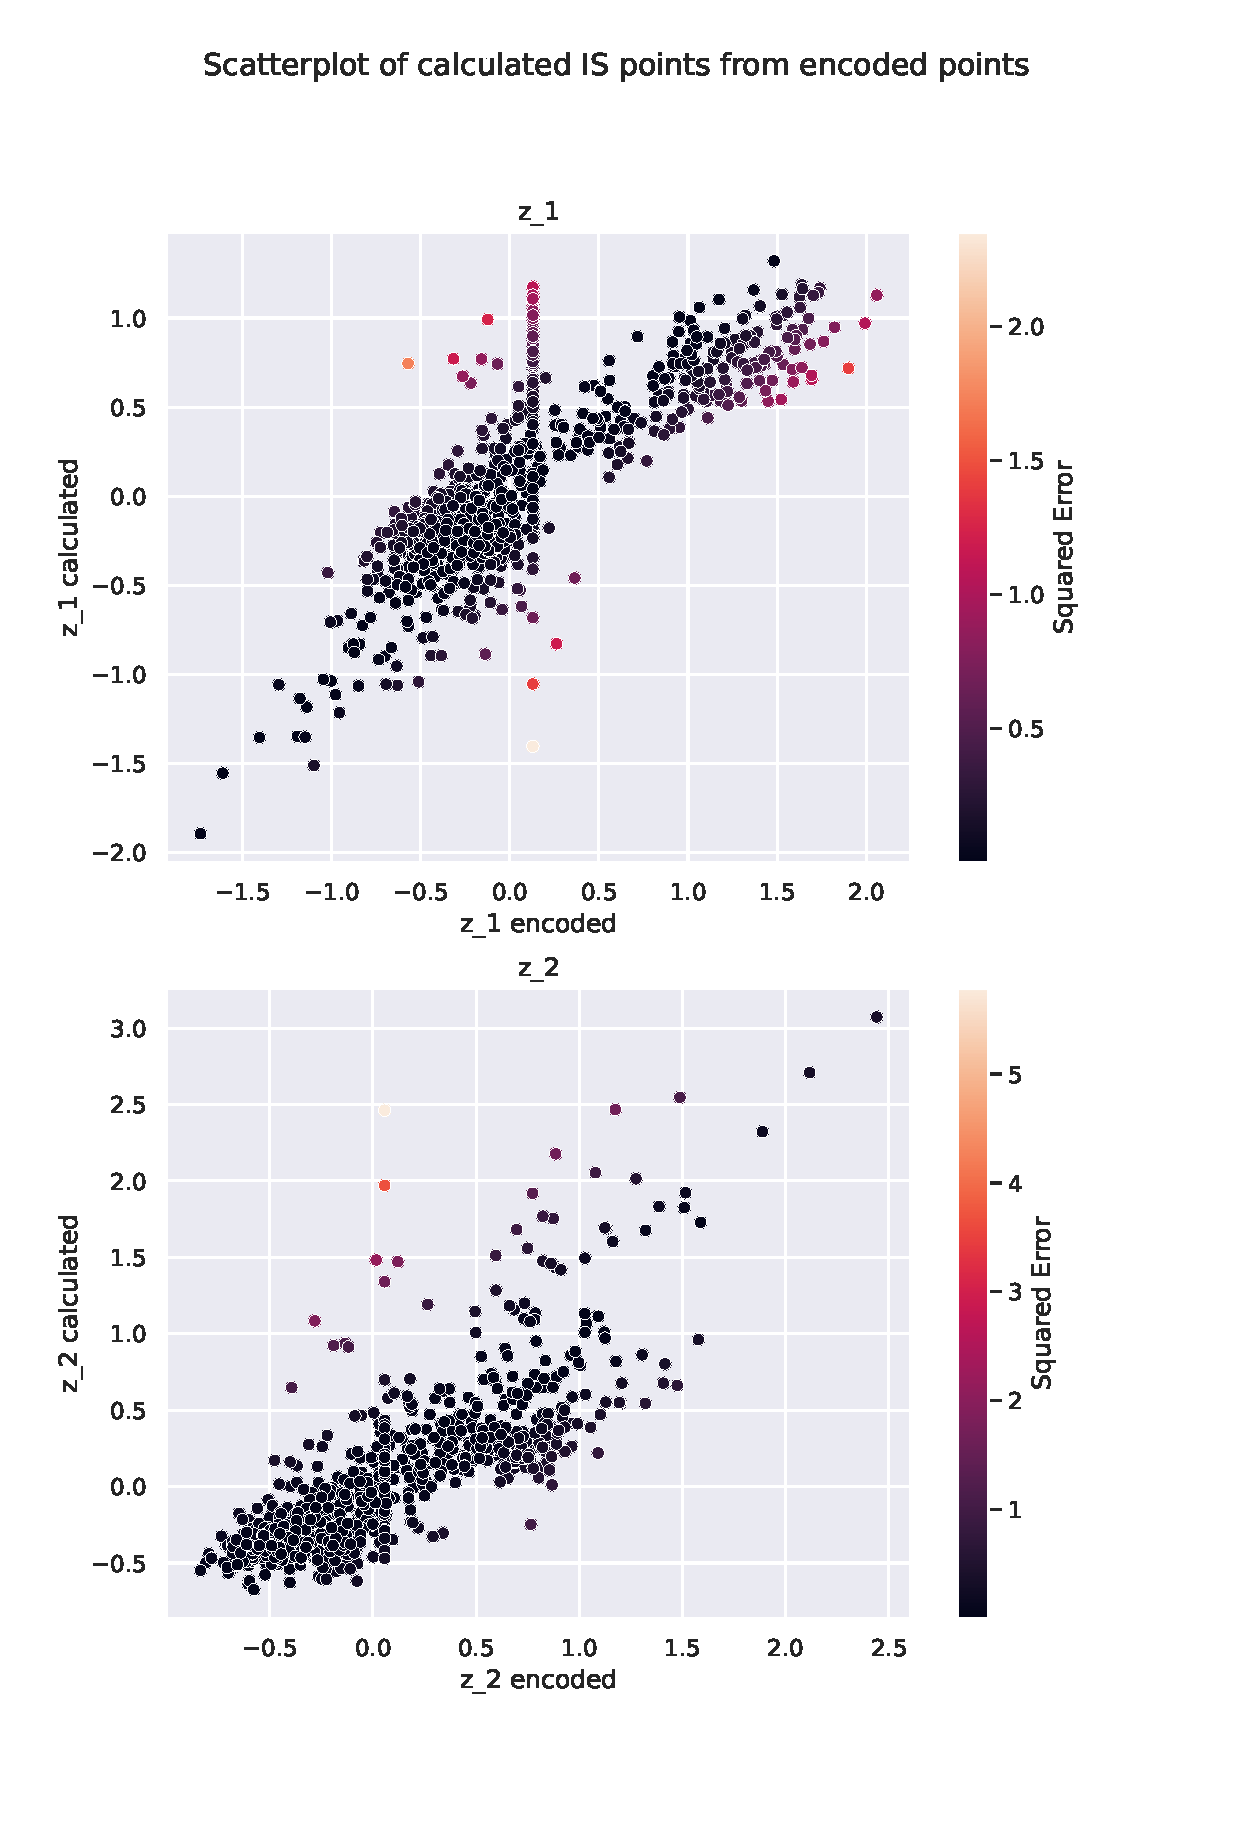
\includegraphics[width=0.7\textwidth]{Cap5/scatterplot_enc2}
    \caption{Scatterplot of experiment 2 encoder}
    \label{fig:scatter_enc_exp2}
\end{figure}

\subsection{Experiment 3}

In this experiment we have again deepened the network, with 8 layers and list of features $[1024, 1024, 256, 128, 32, 16, 8, 4]$. The optimizer parameters and training epochs are the same as Experiment 2. The training epoch loss results from TensorBoard are shown in Figure \ref{fig:exp3}.

\begin{figure}[H]
    \centering
    \includegraphics[width=0.7\textwidth]{Cap5/loss_exp3}
    \caption{Experiment 3 training epoch loss}
    \label{fig:exp3}
\end{figure}

The loss has again reduced nicely over the training epochs. Figure \ref{fig:is_gen_points3} shows the instance space with the generated points.

\begin{figure}[H]
    \centering
    \includegraphics[width=0.8\textwidth]{Cap5/is_exp3.png}
    \caption{Instance space with generated points of experiment 3}
    \label{fig:is_gen_points3}
\end{figure}


Figure \ref{fig:is_exp3} shows the instance space with the calculated points from the generated meta-features, with Figure \ref{fig:scatter_exp3} showing another scatterplot of the dimensions.

\begin{figure}[H]
    \centering
    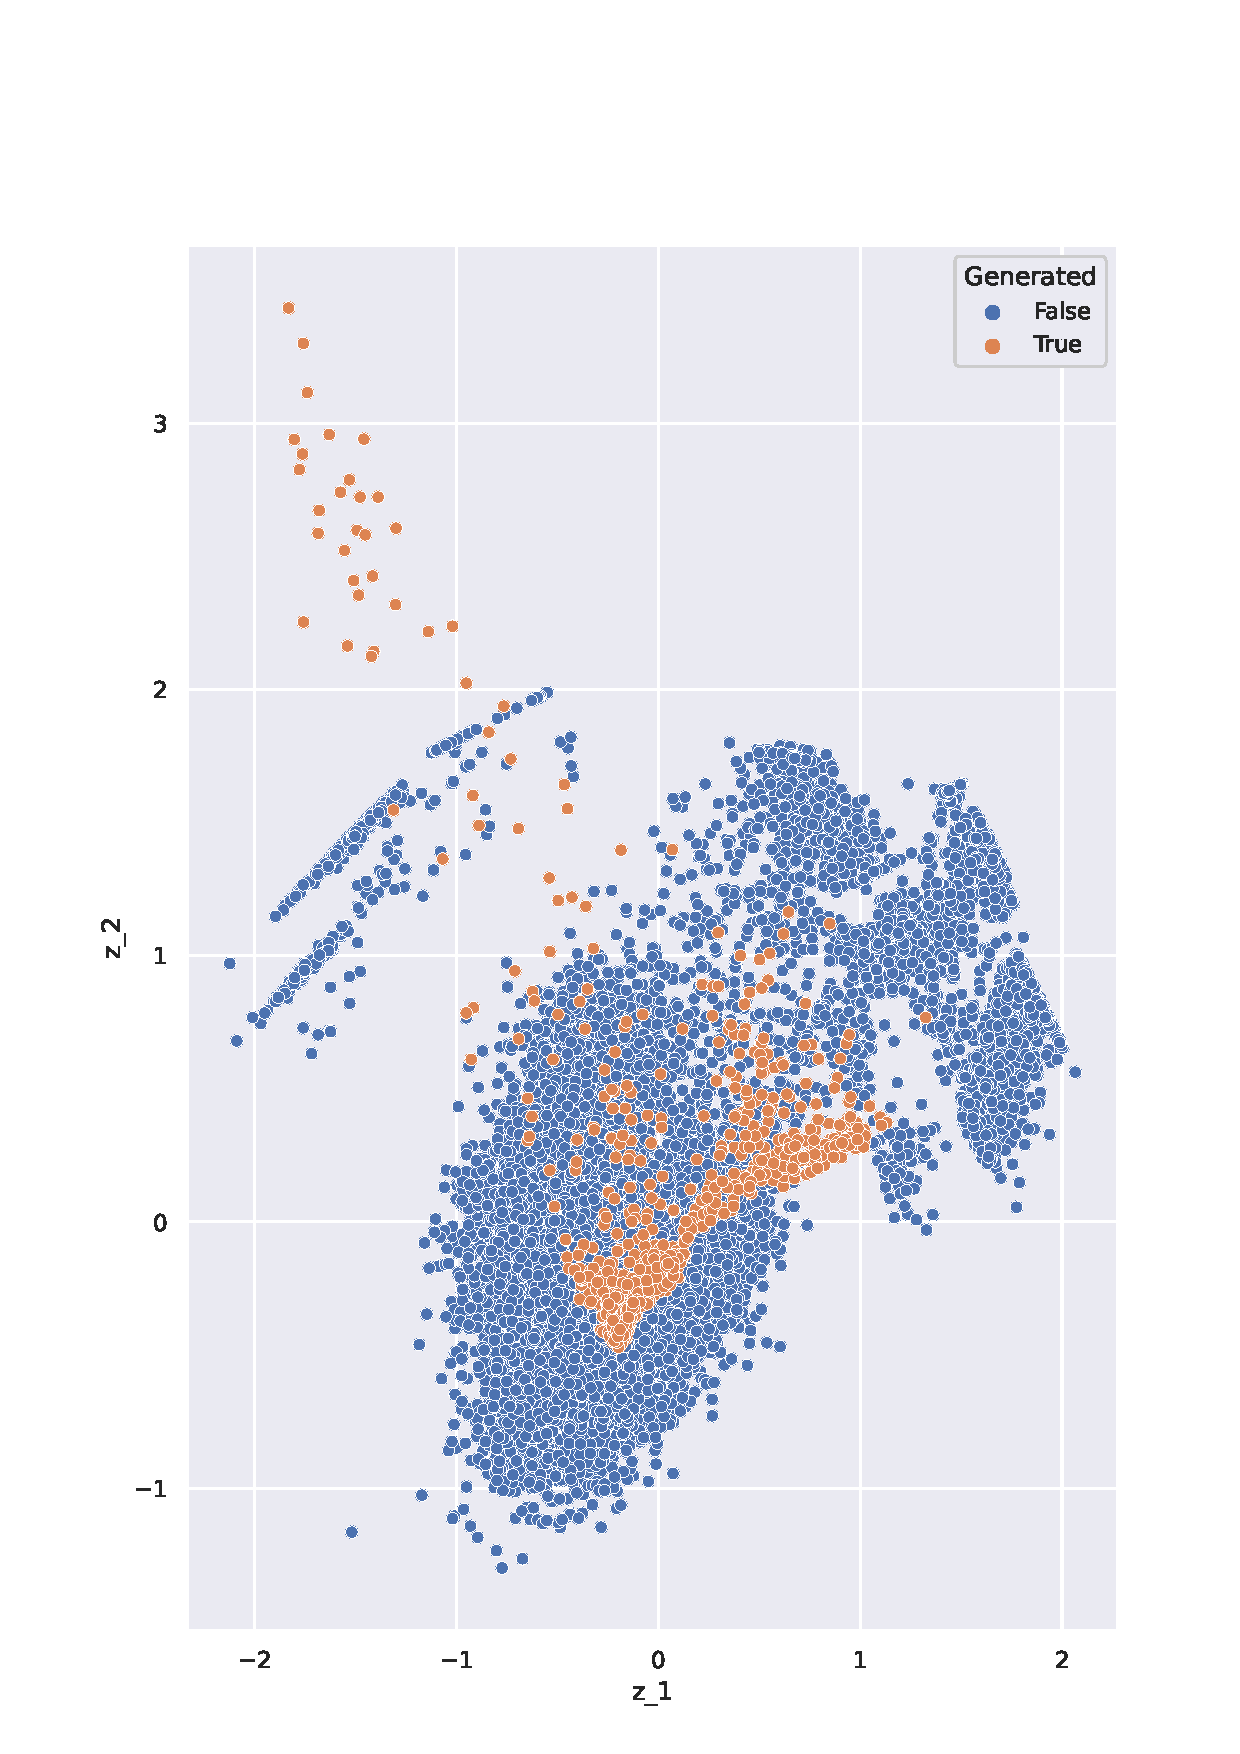
\includegraphics[width=0.8\textwidth]{Cap5/all_coords3.png}
    \caption{Instance space of experiment 3}
    \label{fig:is_exp3}
\end{figure}

\begin{figure}[H]
    \centering
    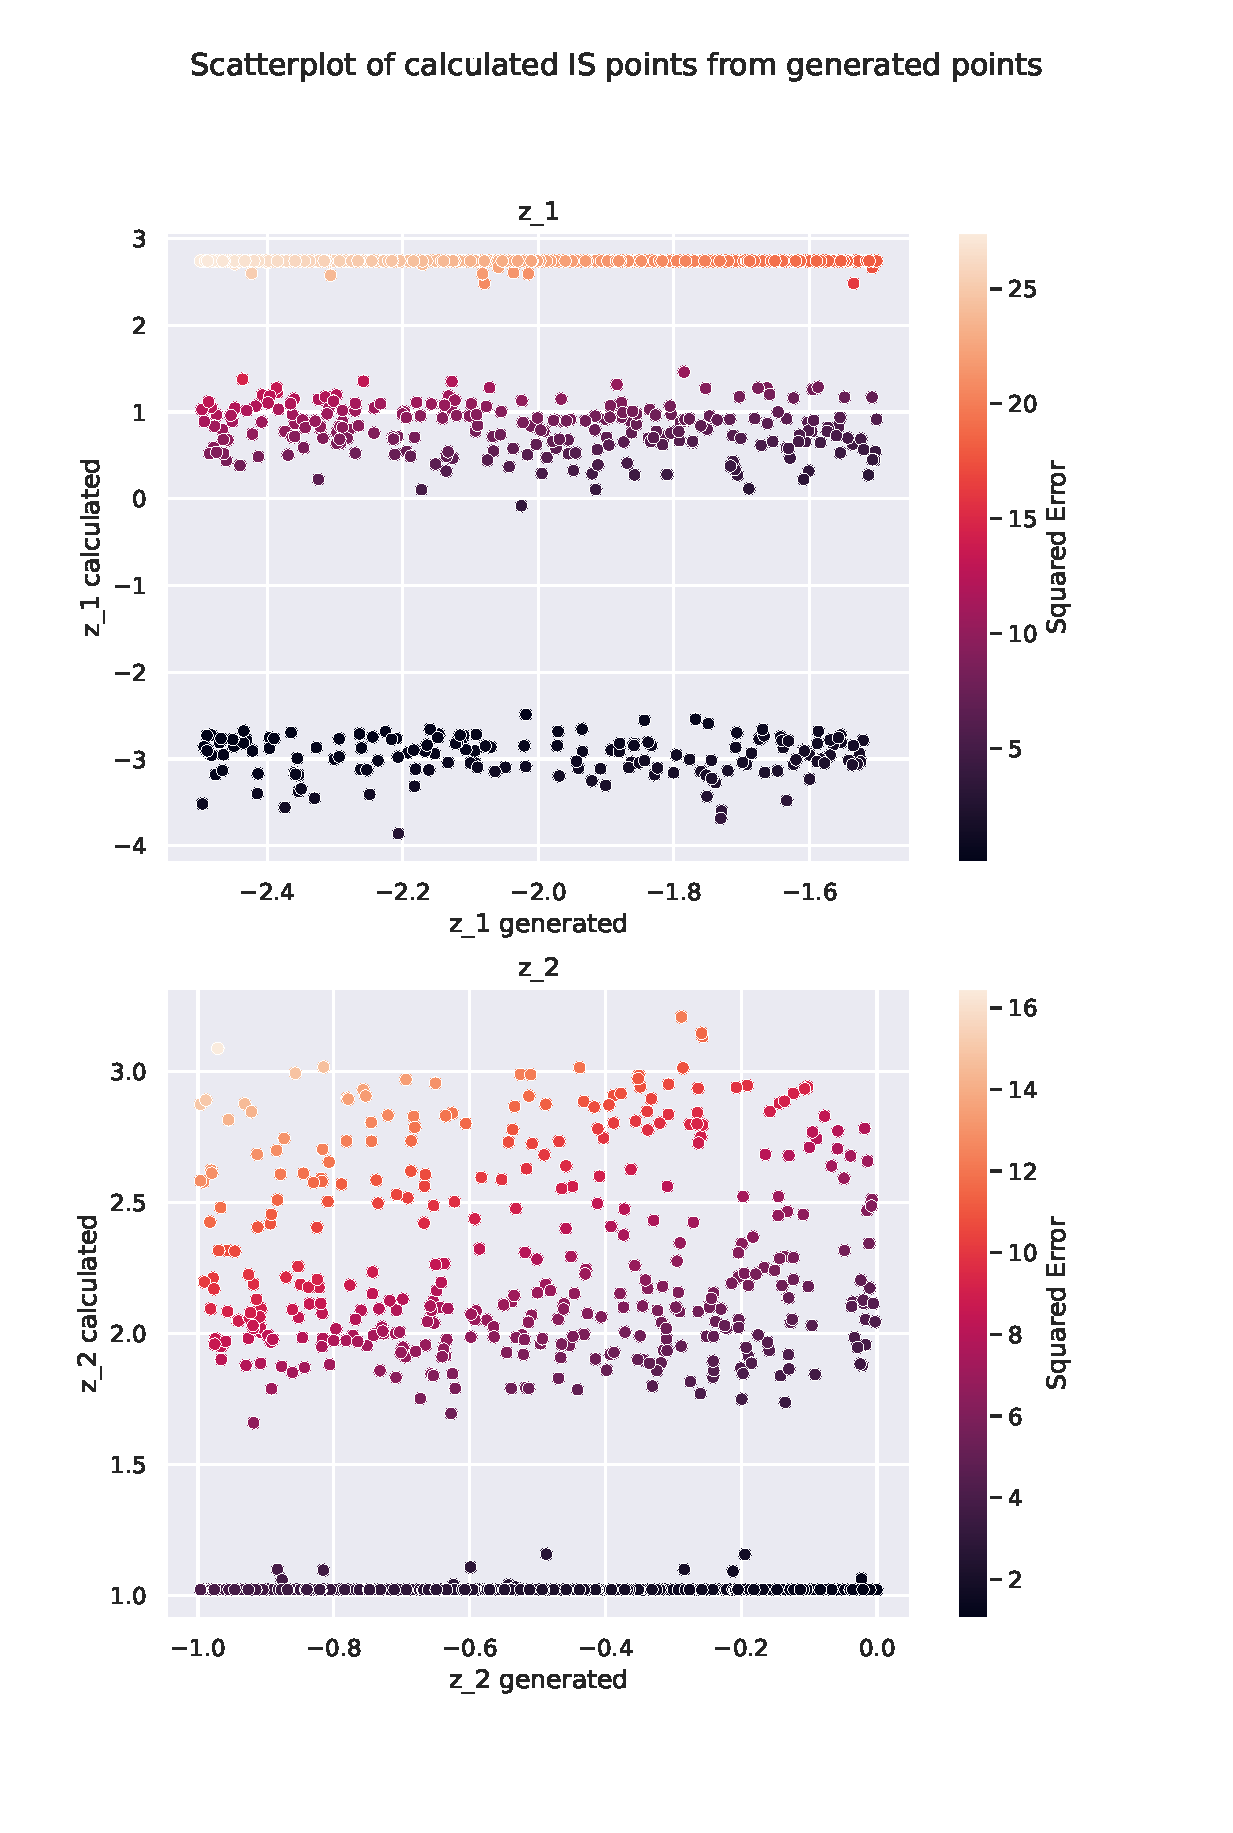
\includegraphics[width=0.7\textwidth]{Cap5/scatterplot3}
    \caption{Scatterplot of experiment 3}
    \label{fig:scatter_exp3}
\end{figure}

Again, most points are uncorrelated with the original values, bunched up in lines. Figure \ref{fig:scatter_enc_exp3} shows the scatterplot for the points returned by the encoder, which are also uncorrelated.

\begin{figure}[H]
    \centering
    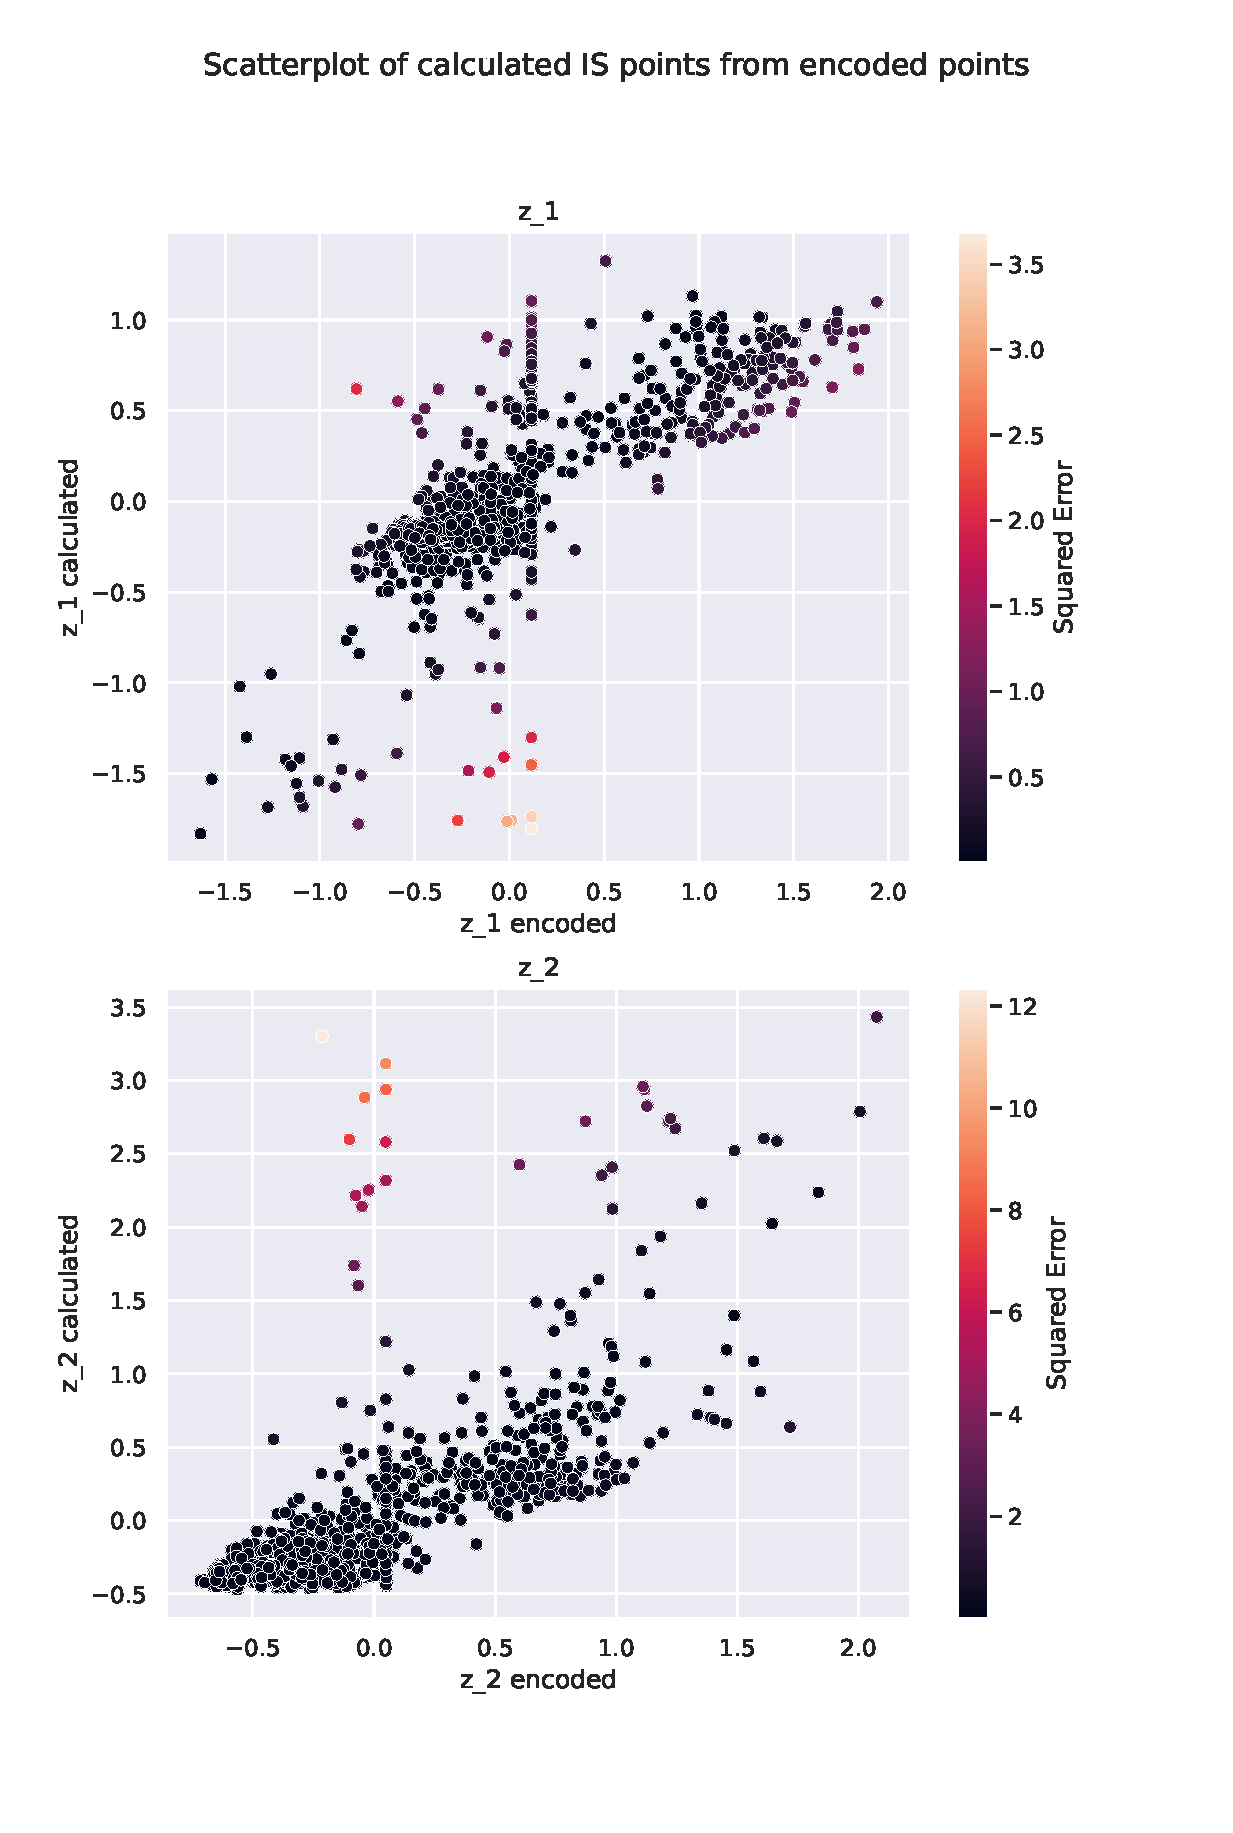
\includegraphics[width=0.7\textwidth]{Cap5/scatterplot_enc3}
    \caption{Scatterplot of experiment 3 encoder}
    \label{fig:scatter_enc_exp3}
\end{figure}